% TODO: Check the right use of the 'collection' and 'document' terms.
% TODO: Get a better understanding about the entity's score in the LingPipe.
% TODO: Create a way to disambiguate the new annotation with the old annotation.
% TODO: More explain on the conversion from new annotation to old annotion.
% TODO: The Java application isn't extendable, report this.

\chapter{Relazione sui compiti svolti}
\label{cap:relazione}

\section{Strutturazione delle attività}
In questo capitolo verranno descritte in modo dettagliato tutte le varie
attività svolte presso la Wonderflow. Ogni sezione raggruppa le mansioni seguite
per realizzare uno specifico prodotto, in modo da esporre in maniera esaustiva
tutte le scelte, gli sviluppi ed i meccanismi messi in atto per portare a
termine il compito.

È da specificare che questo è frutto di un lavoro a posteriori: le varie azioni
conseguite furono pianificate senza una coesione logica e con una certa
discontinuità temporale. Solo a fine esperienza è stato possibile dedurre il
quadro d'insieme, impossibilitando però la produzione di una pianificazione che
seguisse il prodotto dall'inizio alla fine. Anche le stesse mansioni non hanno
sempre potuto godere di una progettazione allegata per via dello scarso
interesse che l'azienda nutre.

\section{Modulo NER}
\subsection{Esportatore annotazioni dalle recensioni}
\subsubsection{Requisiti}
Il funzionamento del modulo NER è strettamente legato al glossario di dove
pesca le annotazioni. Inizialmente il glossario è vuoto quindi i primi risultati
riporteranno la completa assenza di supporto da parte del modulo, ma man mano
che vengano aggiunte nuove annotazioni il sistema d'individuazione inizierà a
svolgere il suo compito. Tuttavia la qualità del servizio nei primi periodi
risentirà della scarsità d'annotazioni raccolte, impedendo di ottenere
suggerimenti che siano un'aiuto concreto all'analista.

Per evitare le basse \textit{performance} iniziali, la Wonderflow ha composto
un insieme di recensioni dove erano presenti annotazioni attentamente
controllate dai \textbf{Senior Analyst} la quale potevano offrire una buona base
di partenza per il glossario.

Il fatto delle annotazioni salvate come attributo della recensione d'origine
però poneva grossi problemi. In primo luogo, ogni programma che gestiva solo
annotazioni avrebbe dovuto conoscere lo schema delle recensioni, creando un
accoppiamento indesiderato; secondo, la semplicità di gestione ed uso
dell'archivio verrebbe meno, principalmente per il fatto di non avere una
relazione \textit{uno a molti} tra annotazione e recensioni.

Necessariamente progettare uno schema che ponesse l'accento sulle annotazioni
piuttosto che sulle recensioni diventava indispensabile. Altro elemento
fondamentale era compiere l'estrazione e la conversione delle annotazioni al
nuovo formato progettato.

Queste due richieste sono state tradotte nella creazione di:
\begin{itemize}
\item Un \gls{DAO} per gestire oggetti \textit{MongoDB} conformi al nuovo schema
dell'annotazione
\item Script \textit{Node.js} che esporta, modifica e salva le annotazione dal
vecchio al nuovo formato
\end{itemize}

La realizzazione di un \gls{DAO} segue sia una norma interna, dove ogni
entità di natura persistente all'interno della compagnia richiede la
realizzazione di un archivio e di un \gls{DAO} associato, sia la sua effettiva
praticità d'uso.

\subsubsection{Sviluppo}
Data la dipendenza dello script con il modulo \gls{DAO} associato alle nuove
annotazioni è stato considerato valido partire con lo sviluppo di quest'ultimo.

La Wonderflow raggruppa i propri \gls{DAO} in un pacchetto \textit{npm} chiamato
``\textit{models}'' in modo che, ogni qualvolta è richiesto l'accesso al
database, sia sufficiente includerlo nel proprio progetto e importare il
\gls{DAO} desiderato. La parte relativa al progetto è illustrata in figura
\ref{fig:dao_annotation}.

\begin{figure}[H]
\begin{center}
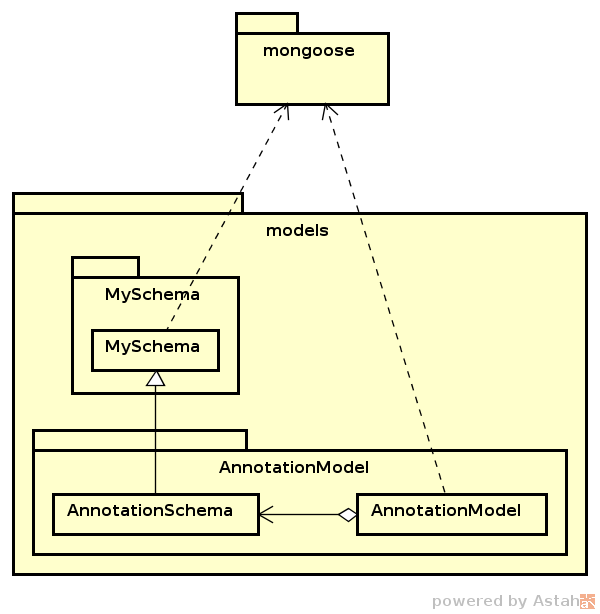
\includegraphics[height=9cm]{dao_annotation}
\caption{
Rappresentazione DAO per le annotazioni nel pacchetto ``\textit{models}''
}
\label{fig:dao_annotation}
\end{center}
\end{figure}

Il package \textit{mongoose} rappresenta il pacchetto \textit{npm} con il quale
vengono implementati i \gls{DAO}. Vi sono due elementi elementi in
\textit{mongoose}: lo \textbf{schema} ed il \textbf{modello}.

Il primo è ciò che rende questo pacchetto molto versatile alla modellazione dei
dati di un'applicazione. Attraverso la definizione di un oggetto in JavaScript è
possibile definire di quali \textbf{attributi} il dato da modellare è composto e
quali metodi il \gls{DAO} ha per interfacciarsi con esso. Nel caso in specie
``\textit{AnnotationSchema}'' definisce come ``annotazione'' un oggetto conforme
al seguente schema:
\begin{center}
\begin{lstlisting}[
  frame=single,
  caption=Schema entità 'annotazione',
  label=valid_annotation]
{
    "uid": "String",
    "name": "String",
    "text": "String",
    "syn": "String",
    "sentiment": 0 | 1,
    "category": "String",
    "reviews": [{
       "id": "String",
       "start": "Number",
       "offset": "Number",
       "origin": "pros" | "cons" | "free-text",
       "version": "String"
    }]
}
\end{lstlisting}
\end{center}

mentre il \gls{DAO} eredita i metodi \textit{CRUD (create, read, update,
delete)}\footnote{Per una maggior trattazione si veda
\url{http://coursework.vschool.io/mongoose-crud/}}, implementati dal
``\textit{model}'' base di \textit{mongoose}, ed il metodo per effettuare la
connessione al database da ``\textit{MySchema}''. Inoltre aggiunge un
ulteriore metodo di classe: ``\textit{insertOrMerge}''.

La descrizione del metodo verrà approfondita in seguito.

Come si può notare il nuovo schema dell'annotazione è molto simile a quello
risultante dal processo d'analisi, discusso nella sezione
\ref{subsec:processo_recensioni_annotazioni}, ma vi sono alcune differenze che
risolvono egregiamente tutte le problematiche riscontrate:
\begin{itemize}
\item L'annotazione non è più un attributo ma copre il ruolo d'oggetto unico
\item I riferimenti alla recensione in cui appare l'annotazione vengono salvati
nel campo ``\textit{reviews}''
\end{itemize}

Con la prima modifica si rimuove l'accoppiamento indesiderato con la recensione.
Ora un qualsiasi programma che avesse esclusivamente bisogno delle annotazioni
non è vincolato a conoscere la struttura delle recensioni.

Con la seconda modifica invece gira la relazione \textit{uno a molti} tra
la recensione e l'annotazione, ottenendo che nell'annotazione si mantengono i
riferimenti alle recensioni in cui appare. La gestione dei riferimenti è
compito del \textit{insertOrMerge} citato sopra. La sua funzione è di o inserire
la nuova annotazione se non è già presente o di agganciare i riferimenti alle
recensioni non ancora presenti nell'attributo ``\textit{reviews}'', mantenendo
cosi la relazione desiderata.

L'ultimo aspetto da chiarire è il \textbf{modello} di \textit{mongoose},
implementato dalla classe ``AnnotationModel''. Il modello, attraverso lo schema,
funge da costruttore per oggetti legati ad un documento \textit{MongoDB} e
provvisti di tutti i metodi per interfacciarsi. In breve, il modello è il
costruttore dei \gls{DAO}. Nel caso di ``AnnotationModel'' i \gls{DAO}
costruiti sono inerenti alle annotazioni e legati alla collezione
``\textit{Annotation}''. \\

Una volta completata la parte per accedere e manipolare documenti relativi
alla nuova struttura dell'annotazione, si è prodotto lo \gls{script} per
estrarre le annotazioni già presenti nell'archivio aziendale. Il riassunto del
processo è illustrato in figura \ref{fig:extractor_annotation}.

\begin{figure}[H]
\begin{center}
\includegraphics[height=6cm]{extractor_annotation}
\caption{
Rappresentazione processo d'estrazione e trasformazione delle annotazioni
}
\label{fig:extractor_annotation}
\end{center}
\end{figure}

Lo script è organizzato sottoforma di \gls{pipeline} sfruttando l'interfaccia
``\textit{stream}'' di \textit{Node.js} e la libreria \textit{through2}. La
\gls{pipeline} è composta da tre elementi:
\begin{itemize}
\item ReaderData - legge le recensioni dentro l'archivio e crea lo
\textit{stream}
\item AnnotationExtractor - estrae e applica le debite trasformazioni alle
annotazioni
\item AnnotationWriter - scrive le annotazioni nell'archivio
\end{itemize}

Il ``ReaderData'' usa il \gls{DAO} apposito per le recensioni per leggerle tutte
e generare uno ``\textit{stream}'' con il quale le invierà, di volta in volta,
all'``AnnotationExtractor'' tramite il metodo \textit{.pipe()}.

Il metodo permette la comunicazione tra le unità consecutive della
\textit{pipeline} attraverso la generazione d'eventi il cui contenuto
trasportato è il risultato dell'unita precedente. Nel caso tra ``ReaderData'' e
``AnnotationExtractor'' il contenuto è la recensione estratta, mentre tra
``AnnotrationExtractor'' e ``AnnotationWriter'' è l'annotazione modificata
conforme allo schema \ref{valid_annotation}.

Quando ``AnnotationExtractor'' riceve la recensione applica l'algoritmo di
trasformazione illustrato nel diagramma d'attività
\ref{fig:extractor_annotation}. La recensione in input immagazzina le
annotazioni nell'attributo ``\textit{feature2sentiment}''. Tutte le recensioni
con la versione diversa da ``v2'' vengono immediatamente scartate, in modo da
non complicare l'algoritmo d'estrazione. Il corpo centrale del diagramma ha lo
scopo di ribaltare la relazione tra recensione ed annotazione. Gli attributi:
\textit{version, start, offset e origin} sono dipendenti dalla recensione in
cui l'annotazione era stata individuata; perciò vengono inglobati in un unico
oggetto, identificato con l'id della recensione e inserito nell'attributo
``\textit{reviews}'' dell'annotazione. Una volta terminate tutte le annotazioni,
il risultato finale viene trasmetto all'unità successiva.

\begin{figure}[H]
\begin{center}
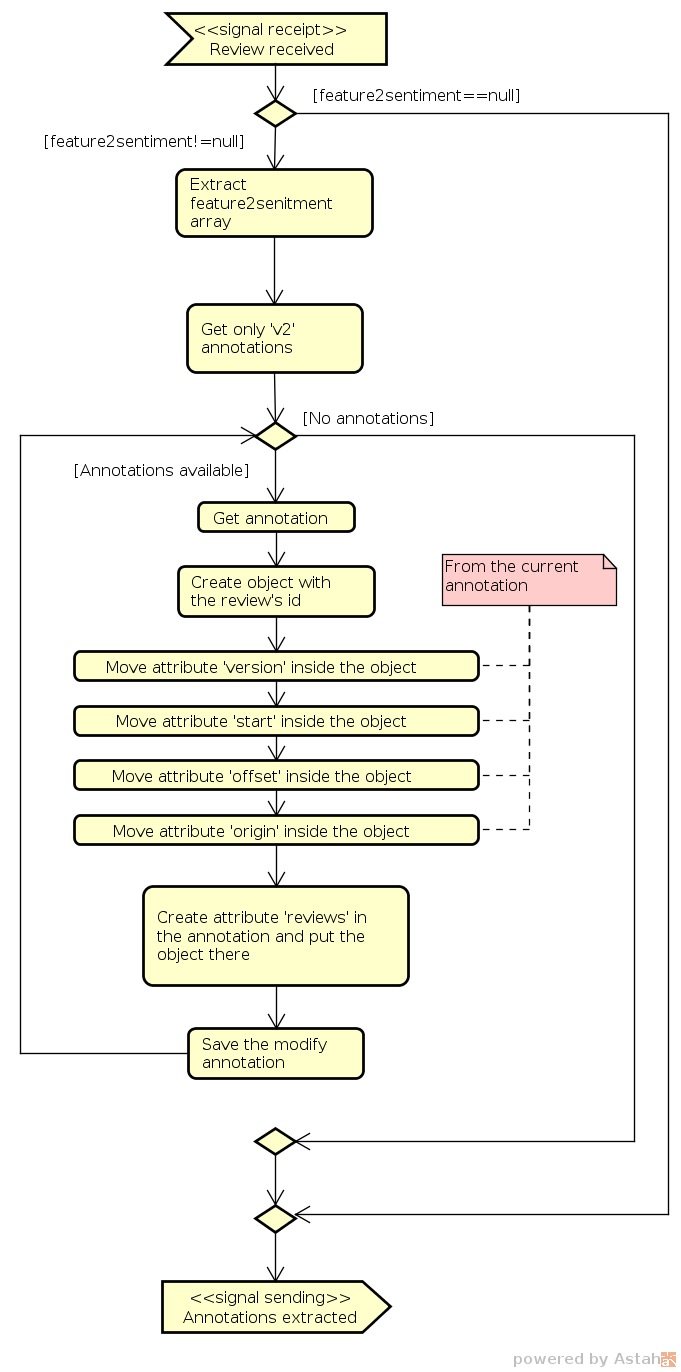
\includegraphics[height=15cm]{extraction_activity}
\caption{
Diagramma d'attività trasformazione annotazioni
}
\label{fig:extraction_activity}
\end{center}
\end{figure}

``AnnotationWriter'' per salvare le annotazioni ricevute nel database, invoca il
metodo \textit{.insertOrMerge()} del \gls{DAO} creato nella fase precedente. In
tal modo, l'unità di scrittura, non dovrà preoccuparsi di come venga mantenuta
la relazione tra annotazioni e recensioni cosi da non violare il
\textit{Single Responsability Principle}.

\subsubsection{Test}
I test svolti nel \gls{DAO} hanno riguardato:
\begin{itemize}
\item L'effettivo salvataggio dell'annotazione
\item La gestione dell'aggiunta della recensione ad un'annotazione che era già
presente nella collezione
\item Controllo che l'aggiunta avvenga solo nel caso di annotazioni uguali.
\end{itemize}

Invece per lo \gls{script} d'estrazione e conversione delle annotazioni è stato
controllato solo se, dato in input un'insieme di recensioni corrette, il
programma terminasse senza alcun errore.

\subsection{Applicazione Java per riconoscere le annotazioni}
\subsubsection{Requisiti}
Il riconoscimento delle annotazioni doveva essere affidato ad un applicazione
Java in modo da usare la libreria \textit{LingPipe} per garantire una certa
efficienza nel portare a termine il compito. Il compito era estendere
un'applicazione Java già esistente, inserendovi le opportune classi per fargli
svolgere il riconoscimento delle annotazioni all'interno di recensioni. In modo
da consentire una rapida integrazione con l'editor messo a disposizione agli
analisti, il formato dell'annotazione doveva essere il medesimo di quello
seguito dall'editor.

Se rispettati questi requisiti, il modulo \gls{NER} si sarebbe integrato nel
sistema complessivo della Wonderflow senza provvedere ad eventuali adattamenti
sia al sistema sia al modulo stesso.

\subsubsection{Sviluppo}
Non si può negare la vastità di tecniche d'analisi del testo che la libreria
\textit{LingPipe} mette a disposizione. Correzione ortografica, identificazione
della lingua, disambiguazione del significato e analista sentimentale sono solo
alcuni dei possibili problemi che si possono affrontare tramite questa libreria
in ambiente Java. Un'altro possibile è proprio la
\textit{Named Entity Recognition}, l'obiettivo del modulo. Attraverso la
documentazione di \textit{LingPipe} i passi per la creazione di un modulo
\gls{NER} risultano molto chiari.

Il sistema di riconoscimento funziona attraverso l'adozione di uno o più metodi
d'individuazione di parole: espressioni regolari, dizionario o modelli
statistici sono quelli citati. In base al metodo scelto si va ad estendere
quella che è la classe usata da \textit{LingPipe} per annotare il testo: il
\textbf{chunk}. Il \textit{chunk} fornisce inoltre un punto d'incontro per tutti
i vari metodi, consentendone un uso simultaneo. Nel progetto di stage non è
stata utilizzata questa proprietà, limitandosi all'uso esclusivo del
\textbf{dizionario}. La scelta è stata compiuta in base al sistema delle
annotazioni precedentemente realizzato, risultando molto semplice adattare i
documenti delle annotazioni in entità per il dizionario. Per sistemi \gls{NER}
\textit{LingPipe} espone l'uso di due tipi di dizionari: quello esatto e quello
approssimato. Nel prima caso, le parole associate a menzioni vengono
riconosciute se coincidono alla forma di com'è stata specificata nel dizionario;
nel secondo, tramite il concetto di \textit{distanza}\footnote{Un esempio è la
\textit{distanza di Levenshtein}} tra due parole, si possono ottenere i
riscontri che si avvicinano, ma non combaciano, alle entità del dizionario.

Come prima versione si è scelto di adottare un dizionario esatto per la sua
facilità d'implementazione e per i discreti risultati che si ottengono, già
verificati dall'azienda.

Parlando delle entità da definire nel dizionario, queste sono coppie di valori
\textit{frase-tipo} seguendo la definizione di \textit{Named entity}. Esse
vengono generate a partire dalle nuove annotazioni la quale, attraverso un
processo di codifica, si forma la coppia richiesta. Ogni qualvolta venga trovata
la frase dell'entità nel testo verrà formato un \textit{chunk} contenente:
la frase stessa, il tipo associato, la posizione di partenza e fine nel testo ed
il punteggio associato all'entità. Per le annotazioni, il tipo non è altro che
la compressione delle informazioni non presenti nel \textit{chunk} al fine di
costruire le annotazioni valide per l'editor. La compressione viene eseguita
ottenendo i campi \textit{uid, category, text, sentiment} e generata la stringa
formata dai rispettivi valori separati dalla guardia ``\$\$\$''. Attraverso il
processo di decodifica del tipo ed i gli altri dati forniti dal \textit{chunk}
si è in grado di costruire un'annotazione che segua lo schema
\ref{snippet_annotation_review} associando:

\begin{enumerate}
\item \textit{category, uid, text} e \textit{sentiment} i valori estratti dal
tipo
\item \textit{name} e \textit{syn} è la frase dell'annotazione
\item \textit{offset} e \textit{start} sono inizializzati attraverso il
\textit{chunk}: il primo sottraendo la posizione di fine \textit{match} con la
posizione d'inizio e l'ultimo assegnandoli la posizione d'inizio
\item \textit{version} viene fissata a ``v2''
\item \textit{origin} è scelta in base al corpo del testo
\end{enumerate}

Come richiesto nei requisiti, l'annotazione risultante possiede l'attributo
\textit{createdBy} inizializzato con il nome della classe che si occupa di
usare i metodi \textit{LingPipe} per eseguire \gls{NER} e di formare
l'annotazione richiesta.

La progettazione dell'applicazione è illustrata in figura
\ref{fig:tag_recognizer}.

``\textit{SentimentMemoryTagRecognizer}'' è la classe che prende le recensioni,
``\textit{TextReviewForAnalytics}'', e genera la lista delle annotazioni,
``\textit{Annotation}'', trovate usando \textit{LingPipe}. Il metodo
\textit{.findTagsInText()} è l'effettivo metodo che riconosce le annotazioni nel
testo e genera la lista delle annotazioni. Essendo che una recensione può essere
divisa in tre parti: testo libero, aspetti positivi e negativi;
\textit{.findTagsInReview()} invoca \textit{.findTagsInText()} e nelle
annotazioni risultate riporta la provenienza.

L'operazione di compressione e decompressione viene svolta da
``\textit{SentimentMemoryAnnotationEncoder}'' che espone i metodi necessari per
effettuare sia la codifica, \textit{.encode()}, sia la codifica,
\textit{.decode()}.

Infine, ``\textit{SentimentMemoryTagRecognizerFactory}'' è una versione del
pattern \textit{Factory Method} dove tutta la logica e complessità
dell'algoritmo di costruzione di un oggetto vengono spostate in un'altra entità
che se ne fa carico. Nel caso attuale, nel \textit{factory} è racchiusa la
costruzione del dizionario, necessario alla costruzione di
``\textit{SentimentMemoryTagRecognizer}'' in modo da applicare la ricerca delle
annotazioni. Trammite l'uso del pattern si ambisce al
\gls{separation_of_concerns}, separando come il dizionario viene creato, svolto
dal ``\textit{SentimentMemoryTagRecognizerFactory}'', e il come viene usato,
definito in ``\textit{SentimentMemoryTagRecognizer}''.

\begin{figure}[H]
\begin{center}
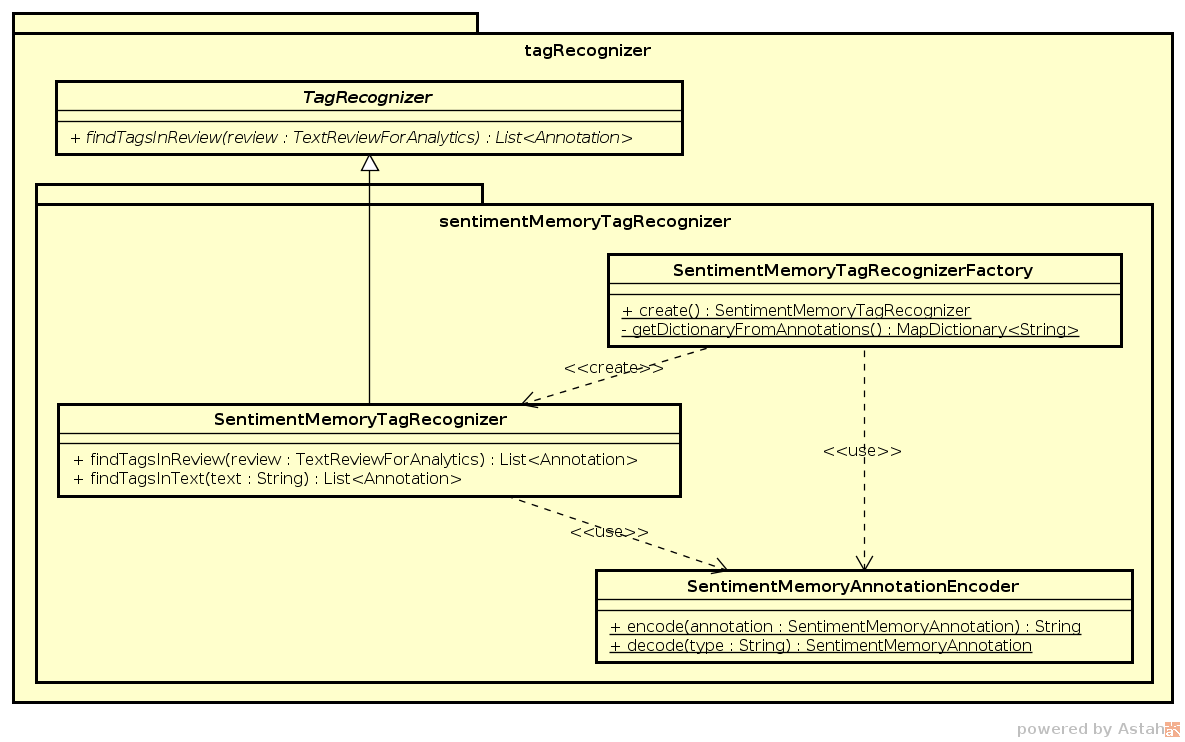
\includegraphics[height=7cm]{tag_recognizer}
\caption{
Diagramma delle classi per il modulo NER
}
\label{fig:tag_recognizer}
\end{center}
\end{figure}

Come era successo nello \gls{script} d'estrazione delle annotazioni, anche qui
si andavano a gestire entità persistenti nell'ecosistema dell'azienda e perciò
si sono implementanti modelli e \gls{DAO} per rappresentarli e gestirli. Le
entità coinvolte nel modulo erano tre: annotazioni del glossario, annotazioni
dell'editor e recensioni. Le ultime due avevano già le classi pronti all'uso,
mentre per il primo è stato necessario realizzarle.

\begin{figure}[H]
\begin{center}
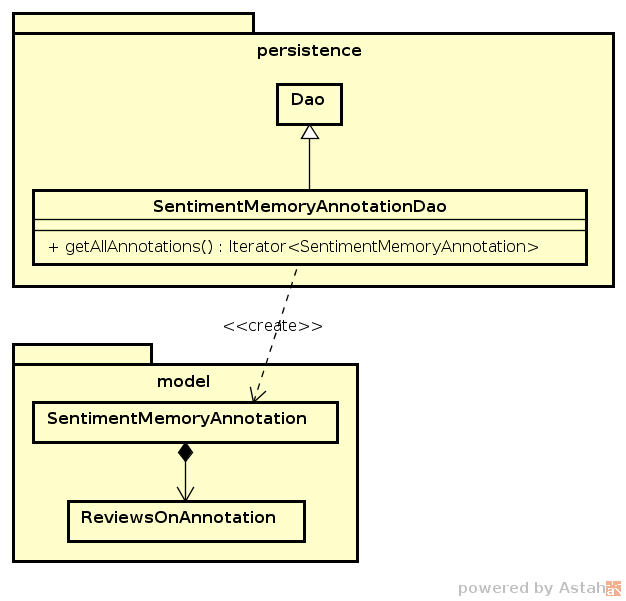
\includegraphics[height=6cm]{model_dao_annotation}
\caption{
Diagramma delle classi per il modello ed il DAO delle annotazioni
}
\label{fig:model_dao_annotation}
\end{center}
\end{figure}

Per implementarle entrambi si è usato la libreria Java \textit{Morphia}, driver
per gestire i documenti di \textit{MongoDB}. Oltre all'accesso effettivo al
database, necessario per realizzare il \gls{DAO}, \textit{Morphia} estende il
sistema delle \textit{annotazioni Java} per mappare classi in documenti in modo
da essere poterli gestire.

Riguardo alle classi create, ``\textit{SentimentMemoryAnnotationDao}'' possiede
il metodo per ottenere tutte le annotazioni del glossario, cosi da poterle
caricare nel dizionario di \textit{LingPipe}; mentre
``\textit{SentimentMemoryAnnotation}'' implementa \textit{getter e setter} per
gli attributi presenti in un'annotazione.

Per effettivamente eseguire il modulo ci pensa un \textit{runner}, il cui altro
non è che una implementazione del \textit{Façade pattern} dove ogni metodo sono
le operazioni eseguibili dall'applicazione Java, compreso il sistema di
riconoscimento delle annotazioni. Sicuramente questo approccio potrebbe
degenerare nella formazione di una \textit{fat interface} ma l'azienda non
prevede l'aggiunta di molte funzionalità al programma. A mio avviso l'uso del
\textit{Command Patter} avrebbe garantito una maggiore estensibilità, senza
introdurre difficoltà progettuali. Il comportamento del \textit{runner} viene
gestito tramite file di configurazione in formato \gls{JSON} dove si vanno a
specifiare:
\begin{itemize}
\item Nome dell'azione da eseguire, attributo \textit{run}
\item Url del database \textit{MongoDB} da utilizzare, attributo
\textit{database}
\end{itemize}

In questa fase non era richiesta l'implementazione del metodo d'avvio del modulo
\gls{NER} perchè sarebbe stata affrontata durante la fase d'integrazione con
l'editor usato dagli analisti.

\subsubsection{Test}
I test sono stati eseguiti sui metodi di
``\textit{SentimentMemoryTagRecognizerFactory}'' e
``\textit{SentimentMemoryTagRecognizer}''.

\paragraph{SentimentMemoryTagRecognizerFactory.create()}
Il test consisteva nella creazione di un'istanza di
``\textit{SentimentMemoryTagRecognizer}'' con associato un dizionario di
annotazioni formato da due elementi caricati precedentemente da una collezione
\textit{MongoDB} in locale. Con \textit{.getDictionary()} di
``\textit{SentimentMemoryTagRecognizer}'' si andava a recuperare il dizionario
per estrarre il numero degli elementi contenuti. Il test passava se la
cardinalità del dizionario coincideva con il numero di annotazioni caricate.

\paragraph{SentimentMemoryTagRecognizer.findTagsInReview()}
Il test iniziava con la compisizione di una recensione modello con le due
caratteristiche
\begin{itemize}
\item Erano defini le tre parti di una recensione: \textit{pros, cons} e
\textit{free-text}
\item Tutte le annotazioni del dizionario erano presenti nelle tre parti.
\end{itemize}
successivamente si eseguiva il metodo \textit{.findTagsInReview()} per ottenere
la lista delle annotazioni. Il test passava quando la lista aveva tanti elementi
quante le annotazioni attese e ogni annotazioni possedeva il campo
\textit{sentiment} e \textit{origin} inizializzato con:
\begin{enumerate}
\item (0, ``cons'') - se l'annotazione provenisse dai \textit{cons} della
recensione
\item (1, ``pros'') - se l'annotazione provenisse dai \textit{pros} della
recensione
\item origin uguale a ``free-text'' se l'annotazione provenisse dal
\textit{free-text} della recensione, l'attributo \textit{sentiment} non viene
controllato
\end{enumerate}

\paragraph{SentimentMemoryTagRecognizer.findTagInText()}
A differenza del test sopra qui si ad assicurare che le annotazioni trovate
siano complete e ogni attributo abbia il giusto valore. Per eseguirlo si è
usata direttamente un testo piano, salvato in una stringa, ed eseguito il metodo
\textit{.findTagInTextTest()} per ottenere la lista di annotazioni presenti.

L'analisi degli attributi veniva eseguita solo su quella in testa alla lista.

\subsection{Integrazione con il tool esistente, l'editor di annotazioni}
\subsubsection{Requisiti}
L'unico requisito espresso è che le annotazioni create attraverso l'applicazione
Java fossero salvate nelle recensioni che si sarebbero andate ad analizzare.
Più precisamente, le annotazioni sarebbero state aggiunte all'array associato
all'attributo \textit{feature2sentiment} della recensione.

\subsubsection{Sviluppo}
Come spiegato nella sezione precedente, per dare la possibilità di avviare il
modulo era sufficiente aggiungere un metodo al \textit{runner} dell'applicazione
che eseguisse l'analisi delle recensioni e salvasse i risultati nel database.

Il metodo è riassunto nell'immagine del diagramma di sequenza
\ref{fig:runner_sequence}.

\begin{figure}[t]
\begin{center}
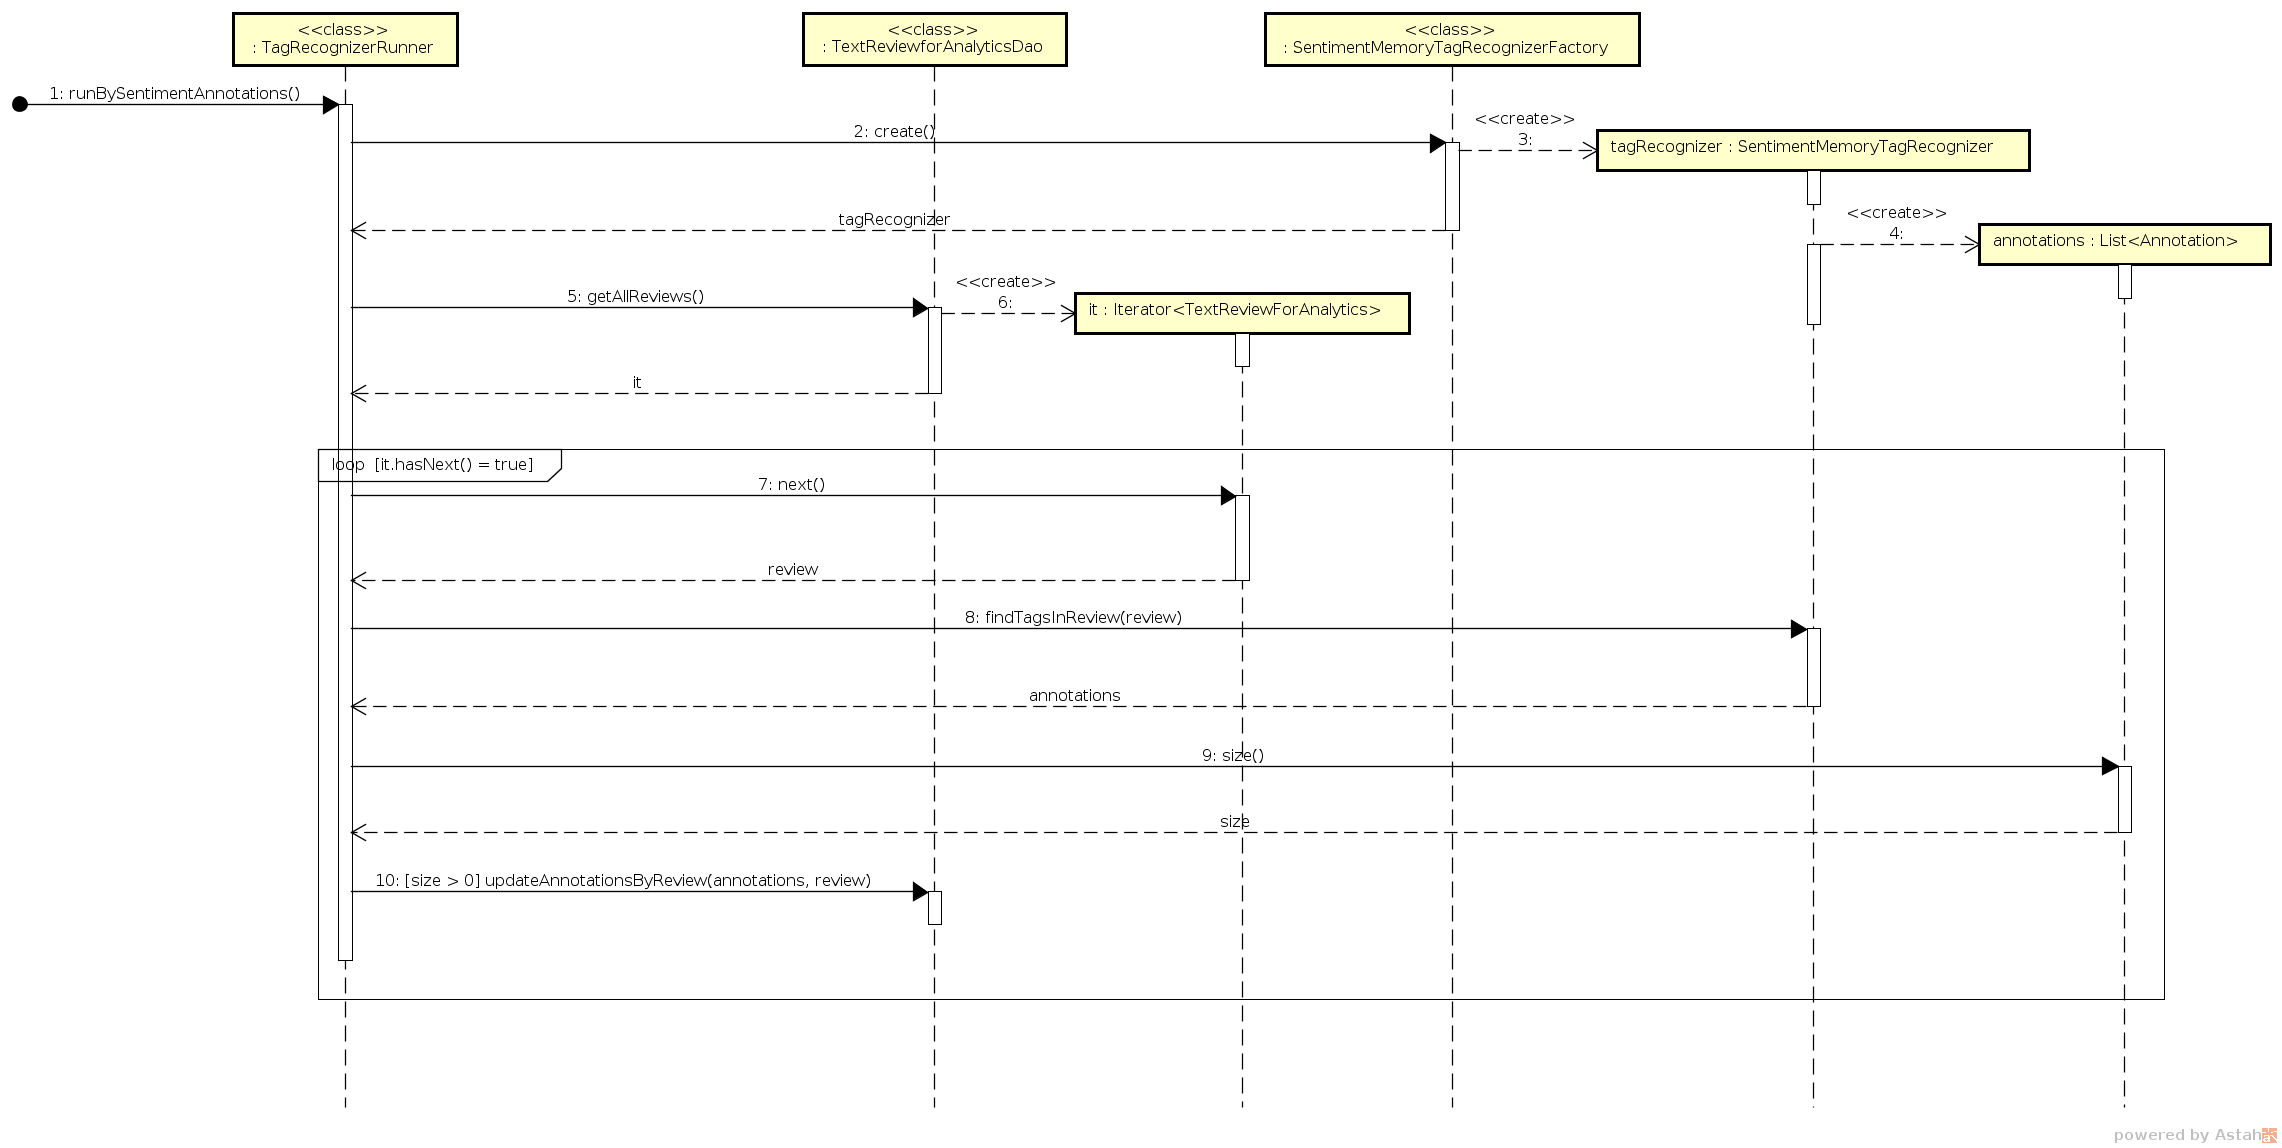
\includegraphics[height=8cm]{runner_sequence}
\caption{
Diagramma di sequenza per il metodo di esecuzione del modulo NER
}
\label{fig:runner_sequence}
\end{center}
\end{figure}

Una volta sviluppato le altre operazioni riguardavano solo il file di
configurazione del modulo \gls{NER}. Nel campo \textit{database} è stato
riportato l'indirizzo del database aziendale dove sono tenute le collezioni
delle recensioni e del glossario; invece in \textit{run} si è trascritto il nome
della \textit{subroutine} di riconoscimento delle annotazioni.

E' da specificare che il processo d'analisi automatica richiede l'intervento
periodico di un operatore umano, in quanto l'azienda non è in possesso di alcun
sistema d'automazione.

\subsubsection{Test}
Non sono stati sviluppati test in quanto le parti che vanno a comporlo sono
state già collaudate e non si è visto la necessità di crearli visto la
dimensione ridotta della funzione. Per quanto riguarda il tool usato dagli
analisti, neanche li vi è stato nessuna creazione di test in quanto il modulo
per l'editor era già stata creato e collaudato precedentemente dall'azienda.

%\subsubsection{Script di misurazione qualità}
%
%\section{Moderazione del glossario}
%\subsection{Comunicazione con il backend}
%\subsubsection{Funzionamento}
%\subsubsection{Modello dell'annotazione}
%\subsubsection{Ampliamento modello della recensione}
%
%\subsection{Interfaccia web}
%\subsubsection{Requisiti}
%\subsubsection{Sviluppo}
%\subsubsection{Test}
%
%\section{Refactoring del BaaS}
%\subsection{Stato iniziale}
%
%\subsection{Progettazione}
%
%\subsection{Ristrutturazione HTTP Handler}
%\subsubsection{Requisiti}
%\subsubsection{Funzionamento}
%\subsubsection{Test}
%
%\subsection{Ristrutturazione applicazione Express}
%\subsubsection{Requisiti}
%\subsubsection{Funzionamento}
%\subsubsection{Test}
%
%\subsection{Ristrutturazione Wonderflow API}
%\subsubsection{Requisiti}
%\subsubsection{Funzionamento}
%\subsubsection{Test}
%
%\subsection{Collaudo e pubblicazione}
%
%\section{Generatore Yeoman per applicazioni AngularJS}
%\subsection{Requisiti}
%\subsection{Funzionamento}
%\subsection{Test}
%
